\documentclass[12pt, leqno]{article} %% use to set typesize
\input{common}

\usepackage{fontspec}
\usepackage{polyglossia}
\setmonofont{DejaVu Sans Mono}[Scale=MatchLowercase]
\usepackage[outputdir=pdf]{minted}

\providecommand{\tightlist}{%
  \setlength{\itemsep}{0pt}\setlength{\parskip}{0pt}}
\begin{document}



\hdr{2023-04-26}

\section{Computing with constraints}

Recall that our basic problem is
\[\mbox{minimize } \phi(x) \mbox{ s.t. } x \in \Omega\] where the
feasible set \(\Omega\) is defined by equality and inequality conditions
\[\Omega = \{ x \in {\mathbb{R}}^n : c_i(x) = 0, i \in \mathcal{E} \mbox{ and }
    c_i(x) \leq 0, i \in \mathcal{I} \}.\]

In the last lecture, we described three different ways to formulate
constrained optimization problem that allow us to build on techniques we
previously explored from unconstrained optimization and equation
solving:

\begin{enumerate}
\def\labelenumi{\arabic{enumi}.}
\tightlist
\item
  \emph{Constraint elimination} (for equality constraints): Find a
  parameterization \(g : {\mathbb{R}}^{n-m} \rightarrow \Omega\)
  formulations and minimize \(\phi(g(y))\) without constraints. This
  requires that the constraints be simple (e.g.~affine equality
  constraints).
\item
  \emph{Barriers and penalties:} Add a term to the objective function
  depending on some parameter \(\mu\). This term penalizes \(x\) values
  that violate the constraint (penalty methods) or that come close to
  \(\partial \Omega\) from the inside (barrier methods). As
  \(\mu \rightarrow 0\), the unconstrained minimum of the modified
  problems converges to the constrained minimum of the original.
\item
  \emph{Lagrange multipliers}: Add new variables (multipliers)
  corresponding to ``forces'' needed to enforce the constraints. The
  \emph{KKT conditions} are a set of nonlinear equations in the original
  unknowns and the multipliers that characterize constrained stationary
  points.
\end{enumerate}

Our goal now is to sketch how modern constrained optimization algorithms
incorporate these different ways of looking at the problem. A full
treatment is well beyond the scope of the class, but we hope to give you
at least the keywords you will need should you encounter them in a
textbook, paper, or a cocktail party. Ideally, knowing something about
what happens in the algorithms will also help you think about which of
various equivalent formulations of an optimization problem will be more
(or less) friendly to solvers. The plan is to first give a ``lay of the
land'' of different families of algorithms, then to give a more detailed
treatment with the running example of linearly constrained quadratic
programs.

For more details, there are some excellent textbooks in the field; some
texts that I really like from my own shelf include:

\begin{itemize}
\tightlist
\item
  \href{https://link.springer.com/book/10.1007/978-0-387-40065-5}{\emph{Numerical
  Optimization}, Nocedal and Wright}
\item
  \href{https://doi.org/10.1137/1.9781611975604}{\emph{Practical
  Optimization}, Gill, Murray, and Wright}
\item
  \href{http://www.athenasc.com/nonlinbook.html}{\emph{Nonlinear
  Programming}, Bertsekas}
\end{itemize}

\section{Lay of the Land}

As we mentioned before, problems with \emph{inequality} constraints tend
to be more difficult than problems with \emph{equality} constraints
alone, because it involves the combinatorial subproblem of figuring out
which constraints are \emph{active} (a constraint \(c_i(x) \leq 0\) is
active if \(c_i(x) = 0\) at the optimum). Once we have figured out the
set of active constraints, we can reduce an inequality-constrained
problem to an equality-constrained problem. Hence, the purely
equality-constrained case is an important subproblem for
inequality-constrained optimizers, as well as a useful problem class in
its own right.

For problems with only equality constraints, there are several standard
options:

\begin{itemize}
\tightlist
\item
  \emph{Null space methods} deal with linear equality constraints by
  reducing to an unconstrained problem in a lower-dimensional space.
\item
  \emph{Projected gradient methods} deal with simple equality
  constraints by combining a (scaled) gradient step and a projection
  onto a constraint set.
\item
  \emph{Penalty methods} approximately solve an equality-constrained
  problem through an unconstrained problem with an extra term that
  penalizes proposed soutions that violate the constraints. That is, we
  use some constrained minimizer to solve
  \[\mbox{minimize } \phi(x) + \frac{1}{\mu} \sum_{i \in\mathcal{E}} c_i(x)^2.\]
  As \(\mu \rightarrow 0\), the minimizers to these approximate problems
  approach the true minimizer, but the Hessians that we encounter along
  the way become increasingly ill-conditioned (with condition number
  proportional to \(\mu^{-1}\)).
\item
  \emph{KKT solvers} directly tackle the first-order optimality
  conditions (the KKT conditions), simultaneously computing the
  constrained minimizer and the associated Lagrange multipliers.
\item
  \emph{Augmented Lagrangian} methods combine the advantages of penalty
  methods and the advantages of the penalty formulation. In an augmented
  Lagrangian solver, one finds critical points for the augmented
  Lagrangian \[\mathcal{L}(x, \lambda; \mu) =
  \phi(x) + \frac{1}{\mu} \sum_{i \in \mathcal{E}} c_i(x)^2 + \lambda^T c(x)\]
  by alternately adjusting the penalty parameter \(\mu\) and the
  Lagrange multipliers.
\end{itemize}

In the inequality-constrained case, we have

\begin{itemize}
\tightlist
\item
  \emph{Active set methods} solve (or approximately solve) a sequence of
  equality-constrained subproblems, shuffling constraints into and out
  of the proposed working set along the way. These methods are
  particularly attractive when one has a good initial estimate of the
  active set.
\item
  \emph{Projected gradient methods} deal with simple inequality
  constraints by combining a (scaled) gradient step and a projection
  onto a constraint set.
\item
  \emph{Barrier methods} and \emph{penalty methods} add a term to the
  objective function in order to penalize constraint violations or
  near-violations; as in the equality-constrained case, a parameter
  \(\mu\) governs a tradeoff between solution quality and conditioning
  of the Hessian matrix.
\item
  \emph{Interior point methods} solve a sequence of barrier subproblems
  using a continuation strategy, where the barrier or penalty parameter
  \(\mu\) is the continuation parameter. This is one of the most popular
  modern solver strategies, though active set methods may show better
  performance when one ``warm starts'' with a good initial guess for the
  solution and the active set of constraints.
\end{itemize}

As with augmented Lagrangian strategies in the equality-constrained
case, state-of-the art strategies for inequality-constrained problems
often combine approaches, using continuation with respect to a barrier
parameters as a method of determining the active set of constraints in
order to get to an equality-constrained subproblem with a good initial
guess for the solution and the Lagrange multipliers.

The \emph{sequential quadratic programming} (SQP) approach for nonlinear
optimization solves a sequence of linearly-constrained quadratic
optimization problems based on Taylor expansion of the objective and
constraints about each iterate. This generalizes simple Newton iteration
for unconstrained optimization, which similarly solves a sequence of
quadratic optimization problems based on Taylor expansion of the
objective. Linearly-constrained quadratic programming problems are hence
an important subproblem in SQP solvers, as well as being an important
problem class in their own right.

\section{Quadratic programs with equality constraints}

We begin with a simple case of a quadratic objective and linear equality
constraints: \begin{align*}
  \phi(x) &= \frac{1}{2} x^T H x - x^T d \\
  c(x) &= A^T x-b = 0,
\end{align*} where \(H \in {\mathbb{R}}^{n \times n}\) is symmetric and
positive definite \emph{on the null space of \(A^T\)} (it may be
indefinite or singular overall), \(A \in {\mathbb{R}}^{n \times m}\) is
full rank with \(m < n\), and \(b \in {\mathbb{R}}^m\). Not only are
such problems useful in their own right, solvers for these problems are
also helpful building blocks for more sophisticated problems --- just as
minimizing an unconstrained quadratic can be seen as the starting point
for Newton's method for unconstrained optimization.

\begin{minted}{julia}
begin
    # Set up a test problem for linearly-constrained QP (2D so that we can plot)
    H = [4.0  1.0 ;
    	 1.0  4.0 ]
    d = [0.5 ; -2.0]
    A = [1.0 ; 1.0]
    b = [1.0]
    
    ϕ1(xy) = xy'*H*xy/2 - xy'*d
    c1(xy) = A'*x - b
end
\end{minted}

\begin{figure}
\begin{center}
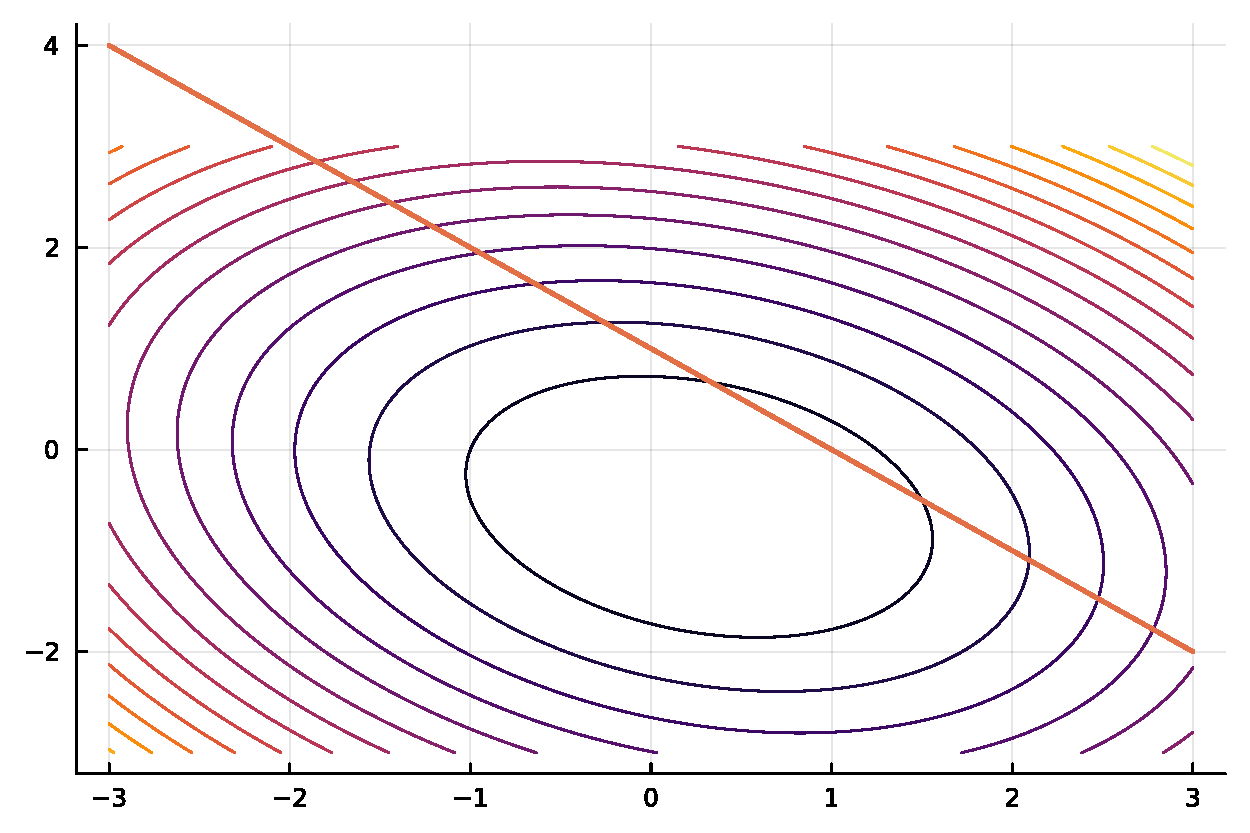
\includegraphics[width=0.8\textwidth]{fig/2023-04-26-test-qp.pdf}
\end{center}
\caption{Example constrained quadratic problem.}
\label{fig:test-qp}
\end{figure}

\subsection{Constraint elimination (linear constraints)}

As discussed last time, we can write the space of solutions to the
constraint equations in terms of a (non-economy) QR decomposition of
\(A\): \[A =
  \begin{bmatrix} Q_1 & Q_2 \end{bmatrix}
  \begin{bmatrix} R_1 \\ 0 \end{bmatrix}\] where \(Q_2\) is a basis for
the null space of \(A^T\). The set of solutions satisfying the
constraints \(A^T x = b\) is
\[\Omega = \{ u + Q_2 y : y \in {\mathbb{R}}^{(n-m)}, u = Q_1 R_1^{-T} b \};\]
here \(u\) is a \emph{particular solution} to the problem. If we
substitute this parameterization of \(\Omega\) into the objective, we
have the unconstrained problem \[\mbox{minimize } \phi(u + Q_2 y).\]
While we can substitute directly to get a quadratic objective in terms
of \(y\), it is easier (and a good exercise in remembering the chain
rule) to compute the stationary equations \begin{align*}
  0
  &= \nabla_y \phi(u + Q_2 y) 
  = \left(\frac{\partial x}{\partial y}\right)^T \nabla_x \phi(u+Q_2 y) \\
  &= Q_2^T (H (Q_2 y + u) - d) 
  = (Q_2^T H Q_2) y - Q_2^T (d-Hu).
\end{align*} In general, even if \(A\) is sparse, \(Q_2\) may be dense,
and so even if \(H\) is dense, we find that \(Q_2^T H Q_2\) is dense.

\begin{minted}{julia}
begin
    # Solve the 2-by-2 problem via a null-space approach
    F = qr(A)
    Q = F.Q * I
    Q1 = Q[:,[1]]
    Q2 = Q[:,[2]]
    
    u_ns = Q1*(F.R'\b)
    H22 = Q2'*H*Q2
    r2  = Q2'*(d-H*u_ns)
    y_ns   = H22\r2
    x_ns   = u_ns + Q2*y_ns
end
\end{minted}

\begin{figure}
\begin{center}
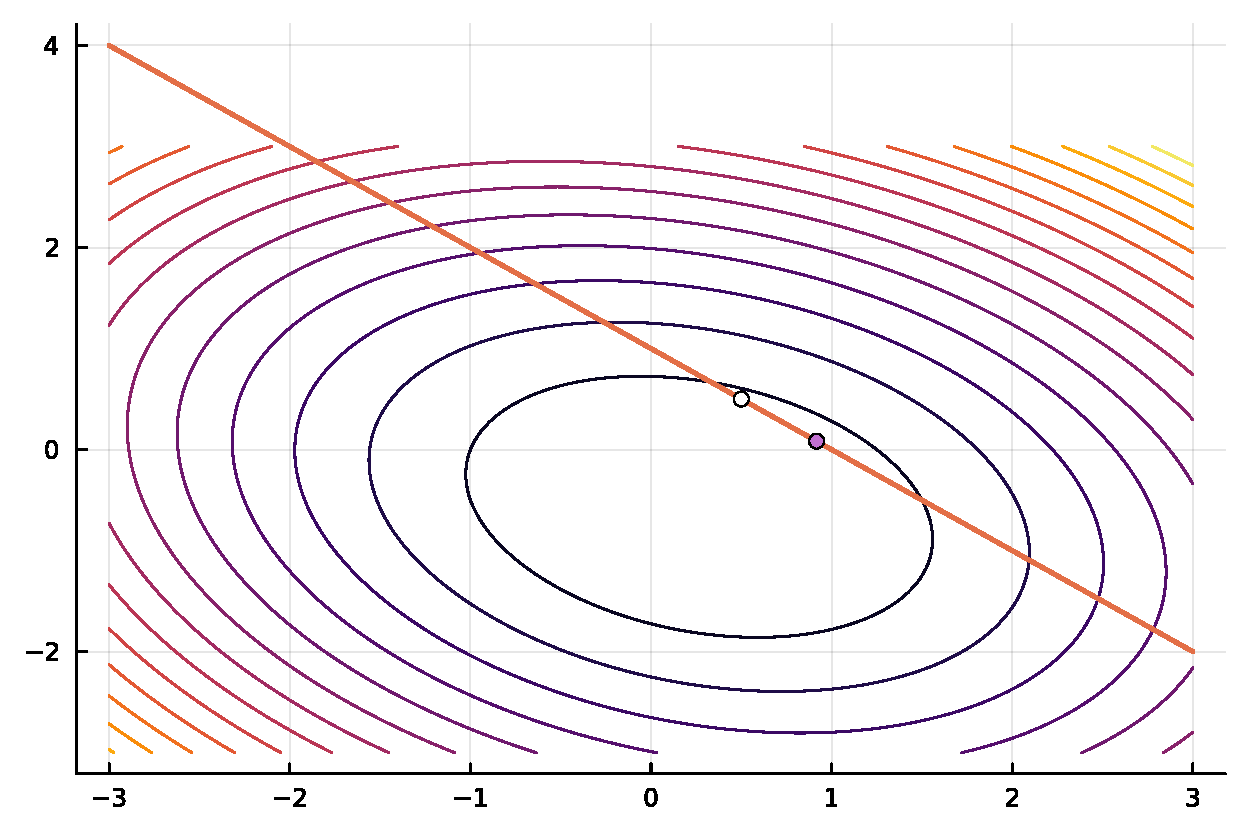
\includegraphics[width=0.8\textwidth]{fig/2023-04-26-qp-ns.pdf}
\end{center}
\caption{Minimization via null space method.  White point is a 
  feasible solution.}
\label{fig:qp-ns}
\end{figure}

The null-space approach is plotted in Figure~\ref{fig:qp-ns}.

Finding a particular solution and a null space basis via QR is great for
numerical stability, but it may not be ideal when the matrices involved
are sparse or structured. An alternative is to use a sparse LU
factorization of \(A^T\):
\[P A^T Q = L \begin{bmatrix} U_1 U_2 \end{bmatrix}.\] where the \(U_1\)
submatrix is upper triangular. A particular solution is then
\[x = Q \begin{bmatrix} U_1^{-1} L^{-1} P b \\ 0 \end{bmatrix}\] and the
null space is spanned by \[Q^T 
  \begin{bmatrix}
    -U_1^{-1} U_2 \\
    I
  \end{bmatrix}.\]

This reformulation may be particularly attractive if \(A\) is large,
sparse, and close to square. Note that pivoting on rectangular
constraint matrices needs to be done carefully, e.g.~using so-called
\emph{rook pivoting} strategies that maintain numerical stability on
full-rank matrices with rank-deficient submatrices.

\subsection{Projected gradient and conjugate gradients}

The \emph{projected gradient} is a variant of gradient descent for
constrained problem. One assumes that we have a projection operator
\(P\) such that \(P(x)\) is the closest point to \(x\) satisfying the
constraint; the iteration is then
\[x_{k+1} = P\left( x_k - \alpha_k \nabla \phi(x_k) \right).\] That is,
we take an (unconstrained) gradient descent step, then project back to
satisfy the constraint. It's an easy enough method to code, provided you
have the projection \(P\).

For our linear equality constraints the projection can be computed by a
least squares type of solve: \begin{align*}
  P(x) &= x + A(A^T A)^{-1} (b-A^T x) \\
       &= (A^T)^\dagger b + (I-AA^\dagger) x \\
       &= (A^T)^\dagger b + (I-\Pi) x
\end{align*} Note that \((A^T)^\dagger b\) is the minimal norm solution
to the constraint equation, and the range space of
\(I-\Pi = I-AA^\dagger\) is the null space of \(A^T\), so this is
similar to the picture we saw with the constraint elimination approach.
And, of course, the gradient in this case is just the residual
\(r_k = Hx_k - d\).

If we start with a point \(x_0\) that is consistent with the
constraints, then each successive point remains on our linear constraint
surface; in this case, we can simplify the iteration to
\[x_{k+1} = x_k - \alpha_k (I-\Pi) r_k.\] This is a stationary iteration
for the underdetermined consistent equation \[(I-\Pi) (Hx_k-d) = 0.\]
Unfortunately, the projected gradient iteration may converge rather
slowly. A tempting thought is to use a scaled version of the gradient,
but the naive version of this iteration will in general converge to the
wrong point unless the projection operator is re-defined in terms of the
distance associated with the same scaling matrix.

If the relevant projection is available, a potentially more attractive
route for this problem is to write \(x = u + z\) for some particular
solution \(u\) (as in the null space approach) and then use a method
like conjugate gradients on the system
\[(I-\Pi) H (I-\Pi) z = (I-\Pi) (d - Hu).\] It turns out that the Krylov
subspace generated by this iteration remains consistent with the
constraint, and so -- somewhat surprisingly at first glance -- the
method continues to work even though \((I-\Pi) H (I-\Pi)\) is singular.

\begin{minted}{julia}
let
    resid_proj(z) = z-Q1*(Q1'*z)  # Function to apply I-Π
    rhs = resid_proj(d-H*u_ns)    # Compute (I-Π)(d-Hu)

    # Define a 2-by-2 symmetric linear map (I-Π)H(I-Π) from a matvec function
    Afun = LinearMap((z)->resid_proj(H*resid_proj(z)), 2, issymmetric=true)
    
    # Solve the singular system via CG
    u_ns + cg(Afun, rhs)
end
\end{minted}

\subsection{Penalties and conditioning}

Now consider a penalty formulation of the same equality-constrained
optimization function, where the penalty is quadratic:
\[\mbox{minimize } \phi(x) + \frac{1}{2\mu} \|A^T x-b\|^2.\] In fact,
the augmented objective function is again quadratic, and the critical
point equations are \[(H + \mu^{-1} AA^T) x = d + \mu^{-1} A b.\] If
\(\mu\) is small enough and the equality-constrained quadratic program
(QP) has a minimum, then \(H+\mu^{-1} AA^T\) is guaranteed to be
positive definite. This means we can solve via Cholesky; or (if the
linear system is larger) we might use conjugate gradients.

We can analyze this more readily by changing to the \(Q\) basis from the
QR decomposition of \(A\) that we saw in the constraint elimination
approach: \[\begin{bmatrix}
  Q_1^T H Q_1 + \mu^{-1} R_1 R_1^T & Q_1^T H Q_2 \\
  Q_2^T H Q_1 & Q_2^T H Q_2
\end{bmatrix}
(Q^T x) =
\begin{bmatrix}
  Q_1^T d + \mu^{-1} R_1 b \\
  Q_2^T d
\end{bmatrix}\] Taking a Schur complement, we have
\[(\mu^{-1} R_1 R_1^T + F)(Q_1^T x) = \mu^{-1} R_1 b - g\] where
\begin{align*}
  F &= Q_1^T H Q_1 - Q_1^T H Q_2 (Q_2^T H Q_2)^{-1} Q_2^T H Q_1 \\
  g &= [I - Q_1^T H Q_2 (Q_2^T H Q_2)^{-1} Q_2^T] d
\end{align*} As \(\mu \rightarrow 0\), the first row of equations is
dominated by the \(\mu^{-1}\) terms, and we are left with
\[R_1 R_1^T (Q_1^T x) - R_1 b \rightarrow 0\] i.e.~\(Q_1 Q_1^T x\) is
converging to \(u = Q_1 R_1^{-T} b\), the particular solution that we
saw in the case of constraint elimination. Plugging this behavior into
the second equation gives
\[(Q_2^T H Q_2) (Q_2^T x) - Q_2^T (d-Hu) \rightarrow 0,\]
i.e.~\(Q_2^T x\) asymptotically behaves like \(y\) in the previous
example. We need large \(\mu\) to get good results if the constraints
are ill-posed or if \(Q_2^T H Q_2\) is close to singular. But in general
the condition number scales like \(O(\mu^{-1})\), and so large values of
\(\mu\) correspond to problems that are numerically unattractive, as
they may lead to large errors or (for iterative solvers) to slow
convergence.

\begin{minted}{julia}
let
    # Vary penalty to illustrate issues -- uniform improvement
    # with smaller penalty until ill-conditioning kills us
    function penalty_err(μ)
	xhat = (H+A*A'/μ)\(d+A*b[1]/μ)
        norm(xhat-x_ns)
    end
    μs = 10.0.^-(1:14)
    errs = penalty_err.(μs)
    plot(μs, errs, xscale=:log10, yscale=:log10, legend=false)
end
\end{minted}

\begin{figure}
\begin{center}
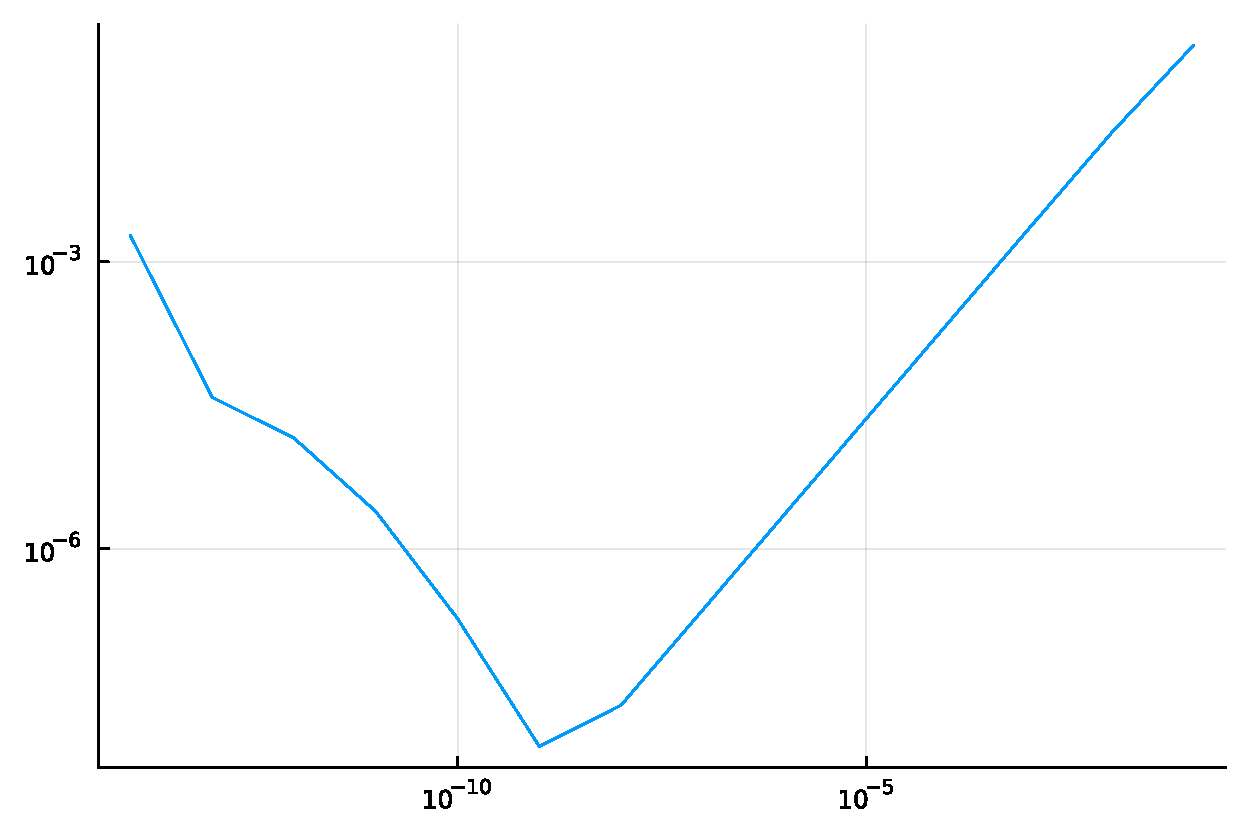
\includegraphics[width=0.8\textwidth]{fig/2023-04-26-penalties.pdf}
\end{center}
\caption{Accuracy as a function of penalty parameters.}
\label{fig:penalties}
\end{figure}

We show the accuracy as a function of penalty parameter
in Figure~\ref{fig:penalties}.  The plot shows the tradeoff between
improving accuracy in exact arithmetic and poor numerical behavior
because of ill conditioning.

\subsection{Lagrange multipliers and KKT systems}

The KKT conditions for our equality-constrained problem say that the
gradient of \[L(x,\lambda) = \phi(x) + \lambda^T (A^T x-b)\] should be
zero. In matrix form, the KKT system (saddle point system)
\[\begin{bmatrix}
    H & A \\
    A^T & 0
  \end{bmatrix}
  \begin{bmatrix} x \\ \lambda \end{bmatrix} =
  \begin{bmatrix} d \\ b \end{bmatrix}.\] If \(A\) and \(H\) are
well-conditioned, then so is this system, so there is no bad numerical
behavior. The system also retains whatever sparsity was present in the
original system matrices \(H\) and \(A\). However, adding the Lagrange
multipliers not only increases the number of variables, but the extended
system lacks any positive definiteness that \(H\) may have.

When there are relatively few constraints and a fast solver with \(H\)
is available, an attractive way to solve this KKT system is the
so-called range-space method, which we recognize as just block Gaussian
elimination: \begin{align*}
  A^T H^{-1} A \lambda &= A^T H^{-1} d - b \\
  x &= H^{-1} (d - A\lambda).
\end{align*} Rewritten as we might implement it, we have \begin{align*}
  H x_0 &= d \\
  H Y   &= A \\
  (A^T Y) \lambda &= A^T x_0 - b \\
  x &= x_0 - Y \lambda.
\end{align*}

The KKT system is closely related to the penalty formulation that we saw
in the previous subsection, in that if we use Gaussian elimination to
remove the variable \(\lambda\) in \[\begin{bmatrix}
    H & A \\
    A^T & -\mu I
  \end{bmatrix}
  \begin{bmatrix} \hat{x} \\ \lambda \end{bmatrix} =
  \begin{bmatrix} d \\ b \end{bmatrix},\] we have the Schur complement
system \[(H+\mu^{-1} AA^T) \hat{x} = d + \mu^{-1} A b,\] which is
identical to the stationary point condition for the quadratically
penalized objective.


\end{document}
